\documentclass[a4paper,11pt]{article}

% Kodovani (cestiny) v dokumentu: utf-8
%\usepackage[cp1250]{inputenc}	% Omezena stredoevropska kodova stranka, pouze MSW.
\usepackage[utf8]{inputenc}	% Doporucujeme pouzivat UTF-8 (unicode).

\usepackage[margin=2cm]{geometry}
\newtoks\jmenopraktika \newtoks\jmeno \newtoks\datum
\newtoks\obor \newtoks\skupina \newtoks\rocnik \newtoks\semestr
\newtoks\cisloulohy \newtoks\jmenoulohy
\newtoks\tlak \newtoks\teplota \newtoks\vlhkost

\jmenopraktika={Fyzikální praktikum 1}
\jmeno={Lukáš Lejdar}
\datum={5. listopadu 2024}
\obor={F}
\skupina={Út 16:00}

\cisloulohy={11}
\jmenoulohy={Interference a difrakce světla}

\tlak={100{,}3}
\teplota={22,5}
\vlhkost={48}

%%%%%%%%%%% Uzitecne balicky:
\usepackage[czech]{babel}

\usepackage{graphicx}
\usepackage{amsmath}
\usepackage{xspace}
\usepackage{url}
\usepackage{indentfirst}
\usepackage{wrapfig}
\usepackage{xcolor}
\usepackage{subfig}
\usepackage{subcaption}
\usepackage{enumitem}
\usepackage{tikzsymbols}
\usepackage{newfloat}

\DeclareFloatingEnvironment[fileext=lof]{graph}
\captionsetup[graph]{labelformat=simple, labelsep=colon, name=Graf}

%%%%%% Zamezeni parchantu:
\widowpenalty 10000 \clubpenalty 10000 \displaywidowpenalty 10000
%%%%%% Parametry pro moznost vsazeni vetsiho poctu obrazku na stranku
\setcounter{topnumber}{3}	  % max. pocet floatu nahore (specifikace t)
\setcounter{bottomnumber}{3}	  % max. pocet floatu dole (specifikace b)
\setcounter{totalnumber}{6}	  % max. pocet floatu na strance celkem
\renewcommand\topfraction{0.9}	  % max podil stranky pro floaty nahore
\renewcommand\bottomfraction{0.9} % max podil stranky pro floaty dole
\renewcommand\textfraction{0.1}	  % min podil stranky, ktery musi obsahovat text
\intextsep=8mm \textfloatsep=8mm  %\intextsep pro ulozeni [h] floatu a \textfloatsep pro [b] or [t]

% Tecky za cisly sekci:
\renewcommand{\thesection}{\arabic{section}.}
\renewcommand{\thesubsection}{\thesection\arabic{subsection}.}
% Jednopismenna mezera mezi cislem a nazvem kapitoly:
\makeatletter \def\@seccntformat#1{\csname the#1\endcsname\hspace{1ex}} \makeatother
%
\newcommand{\vsn}[4]{\ensuremath{#1 =} #2(#3)\,#4}
\newcommand{\vrn}[6]{\ensuremath{#1 =} (#2 $\pm$ #3)\,#4 ($p=$ #5\,\%, $\nu=$ #6)}

\newcommand*\circled[1]{\tikz[baseline=(char.base)]{
		\node[shape=circle,draw,inner sep=1pt] (char) {#1};}}

%%%%%%%%%%%%%%%%%%%%%%%%%%%%%%%%%%%%%%%%%%%%%%%%%%%%%%%%%%%%%%%%%%%%%%%%%%%%%%%
% Zacatek dokumentu
%%%%%%%%%%%%%%%%%%%%%%%%%%%%%%%%%%%%%%%%%%%%%%%%%%%%%%%%%%%%%%%%%%%%%%%%%%%%%%%

\begin{document}

\thispagestyle{empty}

{
\begin{center}
\sf 
{\Large Ústav fyziky a technologií plazmatu Přírodovědecké fakulty Masarykovy univerzity} \\
\bigskip
{\huge \bfseries FYZIKÁLNÍ PRAKTIKUM} \\
\bigskip
{\Large \the\jmenopraktika}
\end{center}

\bigskip

\sf
\noindent
\setlength{\arrayrulewidth}{1pt}
\begin{tabular*}{\textwidth}{@{\extracolsep{\fill}} l l}
\large {\bfseries Zpracoval:}  \the\jmeno & \large  {\bfseries Naměřeno:} \the\datum\\[2mm]
\large  {\bfseries Obor:} \the\obor  \hspace{40mm}  {\bfseries Skupina:} \the\skupina %
&\large {\bfseries Testováno:}\\
\\
\hline
\end{tabular*}
}

\bigskip

{
\sf
\noindent \begin{tabular}{p{4cm} p{0.6\textwidth}}
\Large  Úloha č. {\bfseries \the\cisloulohy:} \par
\smallskip
$T=\the\teplota$~$^\circ$C \par
$p=\the\tlak$~kPa \par
$\varphi=\the\vlhkost$~\%
&\Large \bfseries \the\jmenoulohy  \\[2mm]
\end{tabular}
}

\vskip1cm

\section{Úvod}

V této úloze budu měřit tloušťku tenké hliníkové vrstvy pomocí interference odražených vln a index lomu vzduchu z prodloužení optické dráhy laseru kvůli proměnlivému tlaku. V druhé části budu měřit hustotu vrypů na mřížce z difrakčního obrazce.

\section{Postup měření}

\subsection{Měření tloušťky tenké vrstvy}

Máme skleněnou destičku, napůl pokrytou tenkou hliníkovou vrstvou o neznámé šířce $ t $, na kterou dopadá rovinná monochromatická vlna. Po odrazu vznikají dvě rovnoběžné vlny $ k_{1a} $ a $ k_{1b} $, vzájemně posunuté o fázi $ s = 2 n_{vz} t $. Abychom zjistili posunutí $ s $ a následně i tloušťku $ t $, budeme měřit interferenční obrazec, způsobený třetí vlnou $ k_2 $, šířící se vůči vlnám $ k_{1a} $ a $ k_{1b} $ pod úhlem $ 2 \theta $.

Z podobnosti trojúhelníků ABC a AED na schématickém obrázku 1 dostáváme pro tloušťku vrstvy 

\begin{align}
    t = \frac{x_2}{x_1} \frac{\lambda}{2}.
\end{align}

\begin{table}[htpb]
    \hfill
    \begin{minipage}[b]{.28\linewidth}
        \centering
        \resizebox{\textwidth}{!}{
            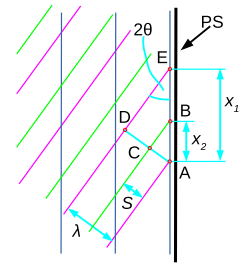
\includegraphics[width=0.28\textwidth]{interference_schema_2.png}
        }
    \end{minipage} 
    \begin{minipage}[b]{.28\linewidth}
        \centering
        \resizebox{\textwidth}{!}{
            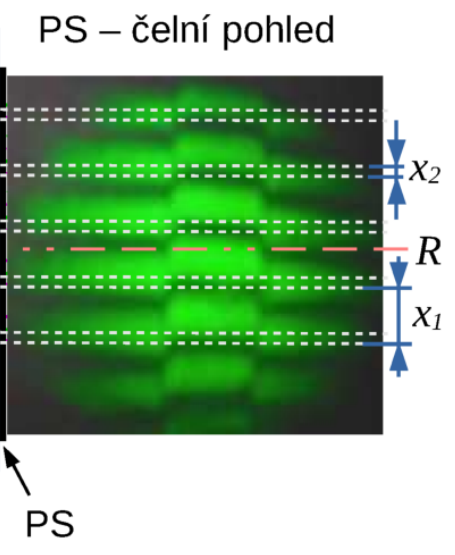
\includegraphics[width=0.28\textwidth]{interference_2.png}
        }
    \end{minipage} 
    \hfill
    \captionsetup{type=figure}
    \caption{Schematické zobrazení interferujících vln: fialová - $ k_{1a} $, zelená - $ k_{1b} $, šedá - $ k_2 $. Pro přehlednost jsou zobrazeny pouze vlnoplochy odpovídající maximům optických polí.}
\end{table}

K realizaci těchto vln využijeme Michelsonova interferometru. Svazek světla ze zdroje (ZS) se rozdělí na polopropustném zrcátku $ DS $, kam se i oba vzniklé svazky znovu vrátí po odrazu na zrcátkách (Z1) a (Z2), a odkud se dál šíří na stínítko (PS). Zrcátko (Z1) je nepatrně nakloněné o úhel $ \theta $ a je na něm položená skleněná destička s vrstvou, na které vznikají odražené vlny $ k_{1a} $ a $ k_{1b} $. Dráze vlny $ k_2 $ odpovídá druhá větev se zrcátkem Z2.

\begin{table}[htpb]
    \begin{minipage}[b]{.45\linewidth}
        \centering
        \resizebox{\textwidth}{!}{ 
            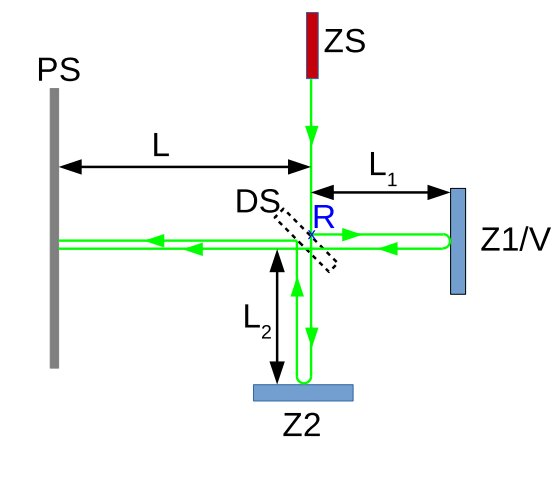
\includegraphics[width=0.4\textwidth]{interferometr_schema.jpg}
        }
    \end{minipage} 
    \hfill
    \begin{minipage}[b]{.45\linewidth}
        \centering
        \resizebox{\textwidth}{!}{ 
            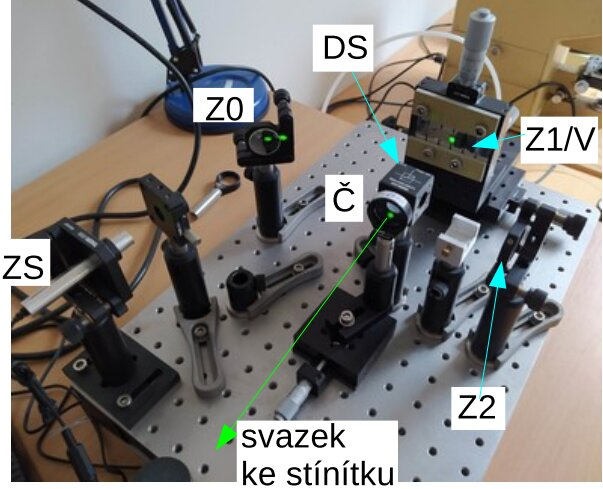
\includegraphics[width=0.4\textwidth]{interferometr.jpg}
        }
    \end{minipage} 
    \captionsetup{type=figure}
    \caption{Schéma Michelsonova interferometru}
\end{table}

\subsection{Určení indexu lomu vzduchu}

K určení indexu lomu vzduchu znovu využijeme Michelsonův interferometr. Do druhého ramene vložím odvzdušněnou kyvetu o délce $ d $ a tlaku $ p_1 $ a postupně ji opět zavzdušňuji. S narůstajícím tlakem se bude měnit optická dráha, což se na stínítku projeví jako pomalu se pohybující interferenční maxima. Index lomu vzduchu se potom dá spočítat jako

\begin{equation}
n = 1 + \frac{N \lambda}{2d} \frac{p_0}{p_0 - p_1},
\end{equation}

\noindent
kde N je počet maxim prošlých kolem nějakého bodu a $ p_1 $ okolní tlak.

\subsection{Měření vzdálenosti vrypů mřížky}

Při difrakci na mřížce se v interferenčním obrazci objevují maxima postupně indexované od středu stínítka počítadlem $ m $. Pro vzdálenost mřížky od stínítka $ x $, mřížkovou konstantu $ d $, vzdálenost m-tého maxima od středu $ y_m $ a vlnovou délku monochromatického světla $ \lambda $ platí

\begin{equation}
d = m \lambda \frac{\sqrt{y_m^2 + x^2} }{y_m}.
\end{equation}

Víme, že maxima se budou objevovat symetricky na obou stranách. Změřím obě vzdálenosti a výsledné $ y_m $ pro m-té maximum vezmu jako jejich průměr

\begin{equation}
y_m =  \frac{y_{m1} + y_{m_2}}{2}
\end{equation}

\newpage

\section{Výsledky měření}

\subsection{Měření tloušťky tenké vrstvy}

Pro deset různých natočení zrcátka (Z2) jsem vyfotil vzniklý interferenční obrazec a digitálně změřil vzdálenosti $ x_1 $ a $ x_2 $. Tyto hodnoty jsem potom dosadil do vztahu (1) a dopočítal konečnou hodnotu $ t $ pro použitý svazek světla o vlnové délce $ \lambda = 532.1 $ nm. Měření jsem provedl jak uprostřed vzorku, tak na jeho okraji, a získal hodnoty

\begin{align*}
   & \text{uprostřed} & t = 88 \pm 7 \text{ nm} & \\
   & \text{na kraji} & t = 85 \pm 9 \text{ nm} && \\
\end{align*}


\begin{table}[htpb]
    \begin{minipage}[b]{.33\linewidth}
        \centering
        \resizebox{\textwidth}{!}{ \includegraphics[trim=300 700 100 500, clip, width=0.3\textwidth]{michelson/PXL_20241105_130927368.jpg} }
    \end{minipage} 
    \begin{minipage}[b]{.33\linewidth}
        \centering
        \resizebox{\textwidth}{!}{ \includegraphics[trim=200 500 200 700, clip, width=0.3\textwidth]{michelson/PXL_20241105_131335487.jpg} }
    \end{minipage} 
    \begin{minipage}[b]{.33\linewidth}
        \centering
        \resizebox{\textwidth}{!}{ \includegraphics[trim=300 600 100 600, clip, width=0.3\textwidth]{michelson/PXL_20241105_131208988.jpg} }
    \end{minipage} 
    \captionsetup{type=figure}
    \caption{Tři z několika vyfocených interferenčních obrazců}
\end{table}

\subsection{Určení indexu lomu vzduchu}

Do druhého ramene Michelsonova experimentu jsem vložil odvzdušněnou kyvetu o délce 40 mm a počítal posun maxim zatímco se kyveta opět zavzdušňovala. Tlak v praktiku bylo $ p_0 = 1003 $ kPa a v odvzdušněné kyvetě vždy zbyl tlak $ p_1 = 103(6) $ kPa. Měření jsem opakoval 4x s laserem o vlnové délce $ \lambda = 532.1 $ nm.

\begin{table}[htpb]
    \centering
    \begin{tabular}{ll}
        N & n \\ \hline\hline
        36.0(4) & 1.00027(3)  \\
        37.0(4) & 1.00027(4) \\
        35.5(4) & 1.00027(4) \\
        36.0(4) & 1.00027(3) \\ \hline
    \end{tabular}
    \caption{Změřený počet prošlých maxim N a výsledné indexy lomu}
\end{table}

Po zprůměrování hodnot jsem obdržel výsledný index lomu vzduchu

\begin{equation}
n_{vz} = 1.00027(6)
\end{equation}

\newpage 

\subsection{Měření vzdálenosti vrypů mřížky}

Zvolenou mřížku jsem umístil na optickou osu ve vzdálenosti od stínítka $ x $ a osvítil ji laserem o vlnové délce $ \lambda = 632.8 $ nm. Pro několik těchto poloh $ x $ jsem odečetl vzdálenosti maxim 1. a 2. řádu a hodnoty uvedl do tabulky 2. Výslednou mřížkovou konstantu $ d $ a hustotu vrypů $ N = \frac{1}{d} $ jsem potom dopočítal dosazením ze vztahů (3) a (4).

\begin{align*}
    d &= 1.66 \pm 0.01 \ \mu \text{m} \\
    N &= 603 \pm 3  \text{ vr mm}^{-1}\\
\end{align*}

\begin{table}[htpb]
    \centering
    \begin{tabular}{r r r r r }
        $ x $ (mm) & $ y_1 $ (mm) & $ y_1' $ (mm) & $ y_2 $ (mm) & $ y_2' $ (mm) \\ \hline \hline
        184(3) & 75.5(3) & 75.5(3) & 202.0(3) & 202.0(3) \\
        165(3) & 68.0(3) & 67.0(3) & 197.0(3) & 196.0(3)  \\
        121(3) & 50.0(3) & 49.5(3) & 144.0(3) & 145.0(3) \\
         96(3) & 40.0(3) & 39.5(3) & 116.5(3) & 117.0(3)  \\
         72(3) & 30.0(3) & 30.5(3) &  87.0(3) &  90.0(3) \\ \hline
    \end{tabular}
    \caption{Měření vzdáleností vrypů mřížky}
\end{table}

\section{Závěr}

Změřil jsem tloušťku tenké hliníkové vrstvy pomocí interferenčního obrazce způsobeného rozdílem fáze vlny odražené na vrstvě a bez ní. Měření jsem opakoval jednou na středu pro hodnotu $ t = 88 \pm 7 $ nm a podruhé na kraji $ t = 85 \pm 9 $.

Pomocí proměnlivé optické dráhy kvůli rostoucímu tlaku v kyvetě jsem určil index lomu vzduchu na $ n_{vz} = 1.00027(6) $, zatímco tabulková hodnota je $ n_{vz} = 1.00026 $. Největším zdrojem nejistoty je nejjednoduché počítání prošlých maxim, které se nepřehledně rozhodí pokaždé když někdo jen projde kolem, nebo se stůl nepatrně zachvěje.

Změřil jsem hustotu vrypů mřížky $ N = 603 \pm 3 $ vr mm$ ^{-1} $ pomocí vzdálenosti interferenčních maxim na stínítku. Tabelovaná hodnota výrobcem je $ N = 600 $ vr mm$ ^{-1} $.

\begin{thebibliography}{0}
\bibitem{tabulky} Návod k úloze ~\url{https://www.physics.muni.cz/praktika/static/navody/fp2/uloha11.pdf}.   
\end{thebibliography}

\end{document}
